%!TEX root =  ../final-report.tex

% Chapters are setup to start on a new page.
% The short version of that title appears in square brackets. This is used for the table of contents listing. 
% The long version of the title has a command "\setstretch{0.5}" in order to reduce the line spacing in the
% title and then the title text.
\chapter[Learning LaTeX]{\setstretch{0.5}Learning LaTeX (example on managing long titles)}
\label{sec:literature}

% Sections will automatically be numbered by LaTeX. 
\section{Sample Section Referencing}
\label{sec:intro:second:section}

% Insert your text in plain text
The report is broken down into chapters, sections, and subsections defined as shown below. The parameter in square brackets is optional and can be used to defined shorter titles to include in the Table of Contents. The labels below each statement are used to link to other parts of the document, such as Sec.~\ref{sec:intro:second:cite}. Similar statements can be used for referencing figures, equations, and tables.
	\begin{verbatim}
		\chapter[Short Name for Table of Contents]{Full Name Shown on Page}
		\label{sec:MyChapterName}
		Sample text reference Sec.~\ref{sec:MyOtherChapter}.
	\end{verbatim}
	\vfill

\section{Sample Citation}
\label{sec:intro:second:cite}
Citations can be managed by in the associated bibtex files and automatically formatted for the IEEE style. Each bibtex item has a unique name associated with it that is used to reference it from the \LaTeX~document. For example, the reference \cite{KeEb95} is created using the code below. 
	\begin{verbatim}
		Some text with a citation \cite{KeEb95}.
	\end{verbatim}

To compile citations, you must compile LaTeX, BibTeX, LaTeX, and LaTeX one more time. The first compilation generates a file listing all the citations in the document (only those used will be listed). The second compile only parses the BibTeX file for the necessary references. The third compile produces the LaTeX code for the references, and the final compile adds the references to your document. 

\section{Sample Equation}
\label{sec:intro:second:equation}
Sample Eq.~\ref{eq:MyEquation}. To learn more about equations, visit \url{http://www.codecogs.com/latex/eqneditor.php}.
\begin{equation}
	A = \pi r^2
	\label{eq:MyEquation}
\end{equation}

Multi-line formula example (particle swarm optimization). Note that the align environment is used to manually break down the equation at logical breaks that enhance readability.
\begin{subequations}
	\label{eq:pso:original}
	\begin{align}
	\textbf{S}_{v,k}\left( n \right) &= \begin{aligned}[t] 
		&\textbf{S}_{v,k} \left( n-1 \right) + \\
		&S_{\varphi1} \times random(0,1) \times \left( \textbf{S}_{p,k} - \textbf{S}_{x,k} \left( n-1 \right) \right) + \\
		&S_{\varphi2} \times random(0,1) \times \left( \textbf{S}_{p,g} - \textbf{S}_{x,k} \left( n-1 \right) \right) 
		\end{aligned} \label{eq:pso:original:velocity} \\
	\textbf{S}_{x,k}\left( n \right) &= \textbf{S}_{x,k}\left( n-1 \right) + \textbf{S}_{v,k} \left( n \right) \label{eq:pso:original:position}
	\end{align}
\end{subequations}\clearpage

\section{Sample Table}
\label{sec:intro:second:table}
This is an example of a table. See Table~\ref{tab:MyTable3}. Tables have many settings and options for merging rows (multirow), merging columns (multicol), and different alignments. The best summary of the common commands is found at \url{http://en.wikibooks.org/wiki/LaTeX/Tables}. In LaTeX, every table border is manually defined. The columns are setup at the beginning of the table, while horizontal lines are manually added at the beginning/end of a row. Notice that cells (columns) are separated by the \& symbol. 

\begin{table}[h]
	\caption{My Table 3}
	\begin{center}
		\begin{tabular}{| l | r | c |}
			\hline
			Sample Row Header & Sample Row Header & Sample Row Header \\\hline
			Left align & Right align & Center align \\\hline
		\end{tabular}
	\end{center}
	\label{tab:MyTable3}
\end{table}%

\begin{table}[h!]
	\caption{My Table 4}
	\begin{center}
		\begin{tabular}{| l | r | c |}
			\hline
			Sample Row Header & Sample Row Header & Sample Row Header \\\hline
			Left align & Right align & Center align \\\hline
		\end{tabular}
	\end{center}
	\label{tab:MyTable4}
\end{table}%


\section{Sample Figure}
\label{sec:intro:second:figure}
Sample Figure~\ref{fig:MyFigure3}. Lorem ipsum dolor sit amet, consectetur adipiscing elit. Pellentesque mattis lectus in velit facilisis lacinia. In eu bibendum lorem. Sed sollicitudin fermentum egestas. Nunc consectetur vehicula orci, eu molestie sapien sollicitudin sit amet. Phasellus sollicitudin sem quis orci aliquet, porta sagittis diam sodales. Suspendisse ullamcorper sollicitudin dictum. Donec quam sapien, molestie ut ullamcorper vitae, porttitor vitae mauris. Quisque ultrices nunc in consectetur malesuada. Pellentesque tristique purus ut felis aliquet pharetra. Mauris posuere lobortis metus id aliquam. Phasellus suscipit sapien vitae leo ultricies suscipit. Vivamus sodales egestas velit sit amet suscipit. Integer libero augue, sodales quis porta commodo, condimentum nec leo. Proin venenatis eros id venenatis facilisis.

Sed adipiscing, risus vitae facilisis egestas, odio mauris sollicitudin diam, at vestibulum eros felis sed arcu. Suspendisse potenti. Sed a quam justo. Suspendisse laoreet eleifend ante, et dapibus odio bibendum nec. Aliquam viverra pellentesque est, auctor fermentum lectus tincidunt in. Praesent hendrerit purus sit amet sodales vehicula. Pellentesque vulputate fermentum justo, eget aliquam urna hendrerit ac. Ut laoreet volutpat iaculis. Duis et erat magna. Vivamus vel neque vel tortor eleifend lobortis nec sed sapien. Duis fermentum vel diam a dignissim. 

Sed adipiscing, risus vitae facilisis egestas, odio mauris sollicitudin diam, at vestibulum eros felis sed arcu. Suspendisse potenti. Sed a quam justo. Suspendisse laoreet eleifend ante, et dapibus odio bibendum nec. Aliquam viverra pellentesque est, auctor fermentum lectus tincidunt in. Praesent hendrerit purus sit amet sodales vehicula. Pellentesque vulputate fermentum justo, eget aliquam urna hendrerit ac. Ut laoreet volutpat iaculis. Duis et erat magna. Vivamus vel neque vel tortor eleifend lobortis nec sed sapien. Duis fermentum vel diam a dignissim. 

% NOTES: Figures should have a width to prevent them from extending past the page margins. 
% The width should be maximum 5.5in.
\begin{figure}[h!]
	\begin{center}
		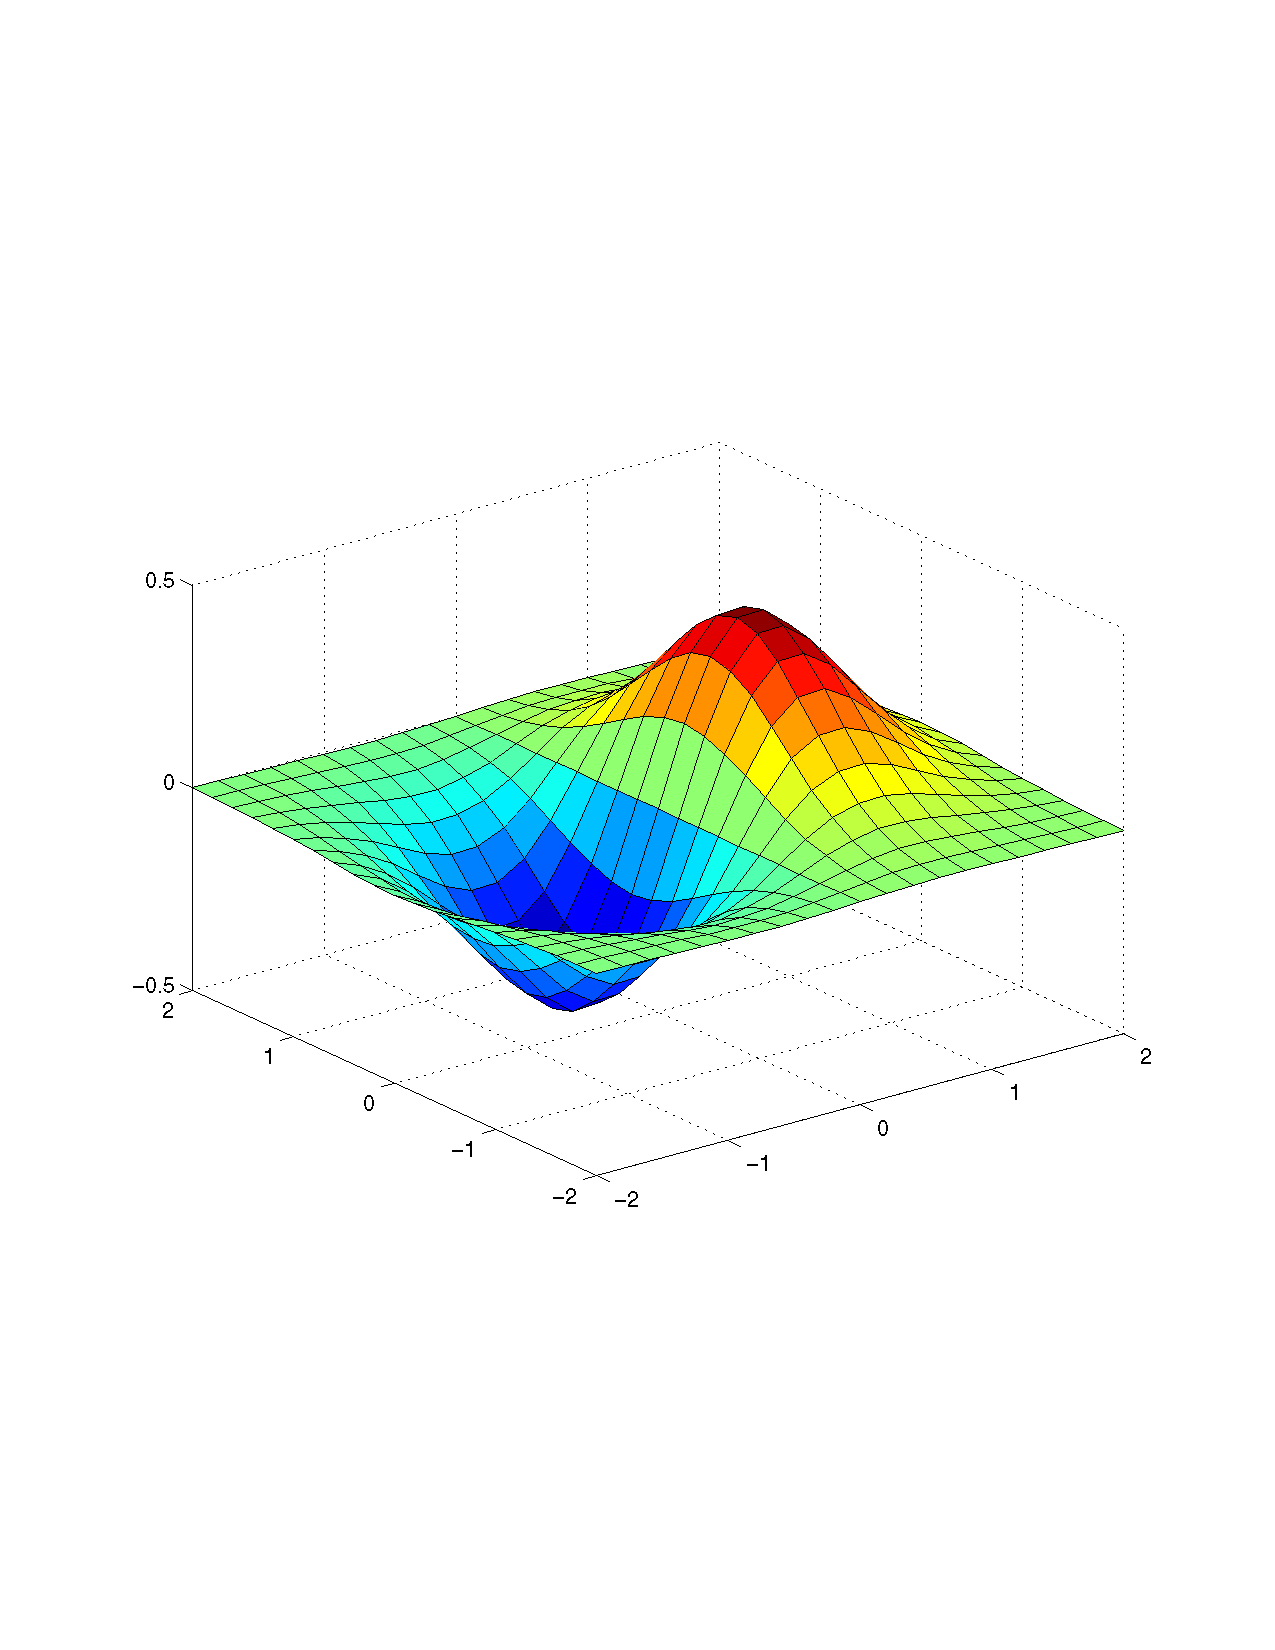
\includegraphics[width=2.5in]{./images/sample.pdf}
		\caption{My Figure 3}
		\label{fig:MyFigure3}
	\end{center}
\end{figure}

Lorem ipsum dolor sit amet, consectetur adipiscing elit. Pellentesque mattis lectus in velit facilisis lacinia. In eu bibendum lorem. Sed sollicitudin fermentum egestas. Nunc consectetur vehicula orci, eu molestie sapien sollicitudin sit amet. Phasellus sollicitudin sem quis orci aliquet, porta sagittis diam sodales. Suspendisse ullamcorper sollicitudin dictum. Donec quam sapien, molestie ut ullamcorper vitae, porttitor vitae mauris. Quisque ultrices nunc in consectetur malesuada. Pellentesque tristique purus ut felis aliquet pharetra. Mauris posuere lobortis metus id aliquam. Phasellus suscipit sapien vitae leo ultricies suscipit. Vivamus sodales egestas velit sit amet suscipit. Integer libero augue, sodales quis porta commodo, condimentum nec leo. Proin venenatis eros id venenatis facilisis.

\begin{figure}[h!]
	\begin{center}
		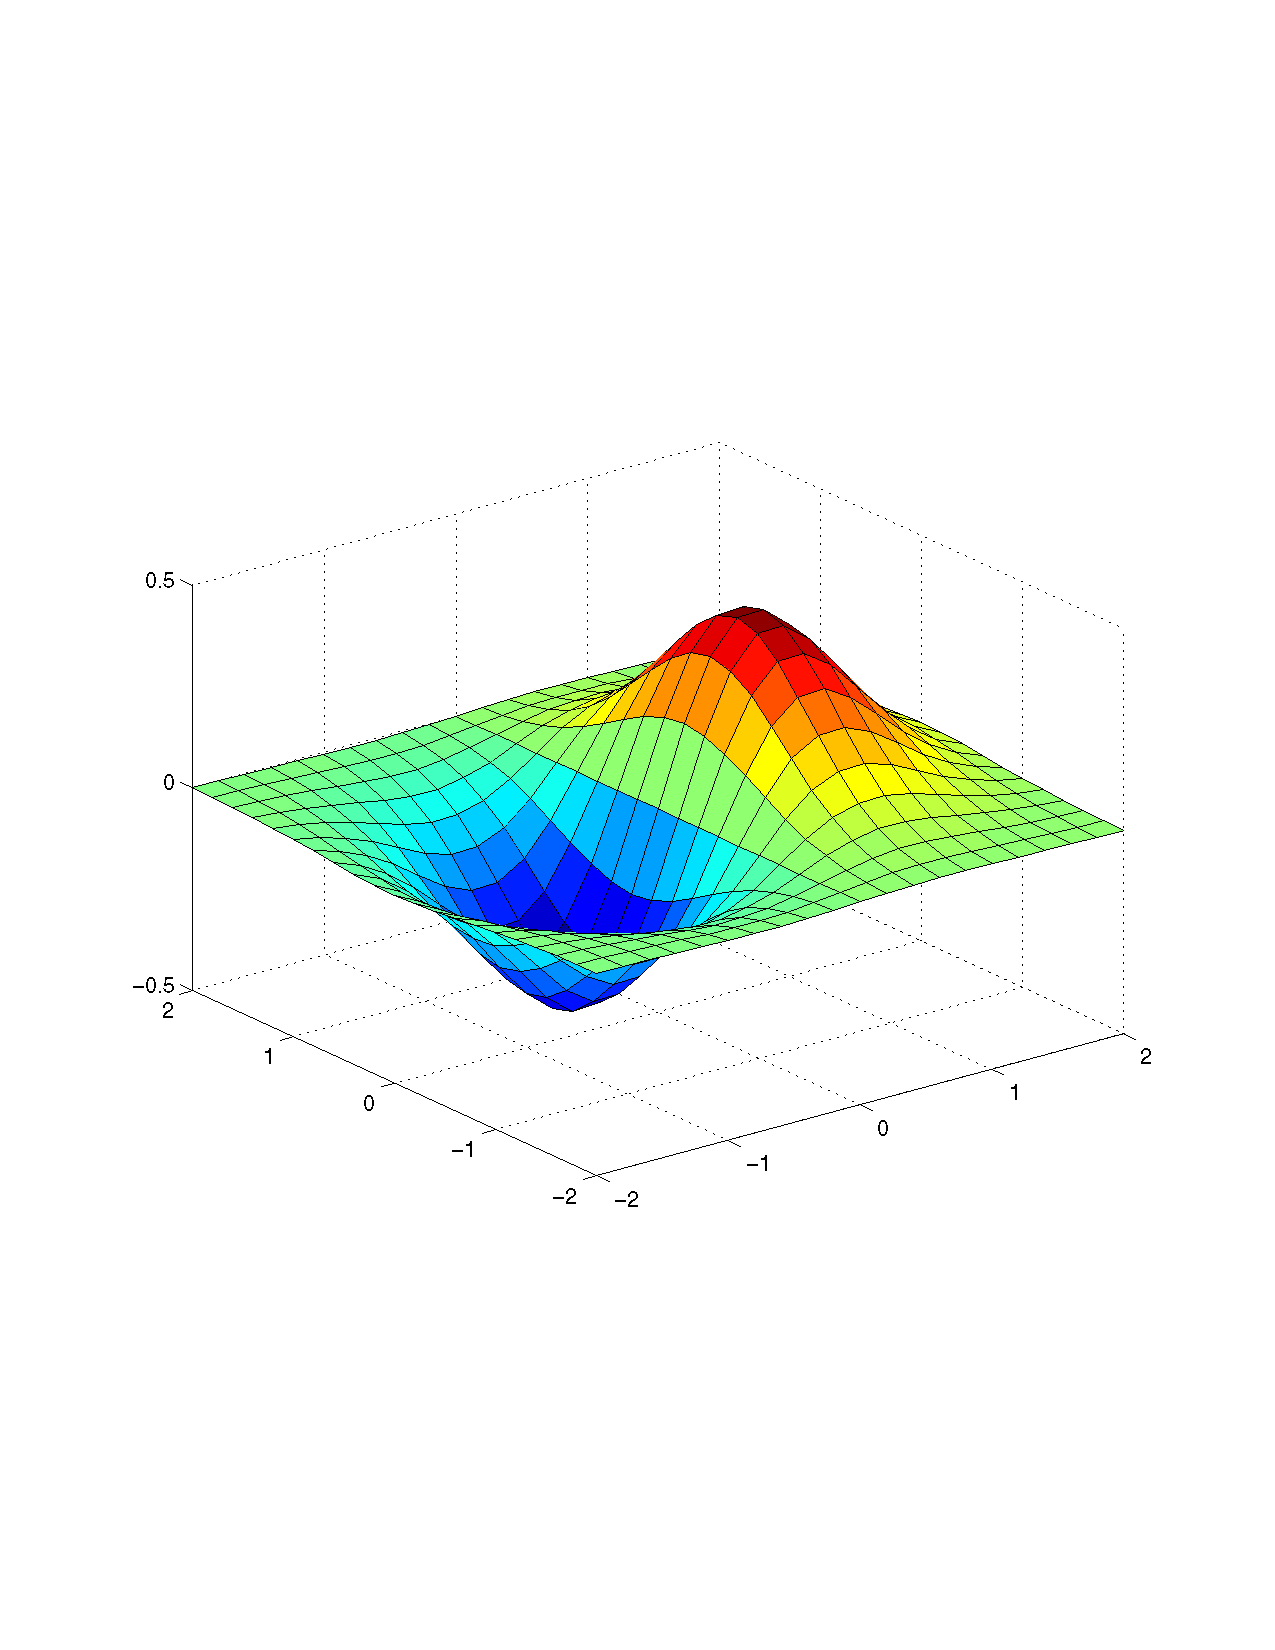
\includegraphics[width=2.5in]{./images/sample.pdf}
		\caption{My Figure 4}
		\label{fig:MyFigure4}
	\end{center}
\end{figure}

Sed adipiscing, risus vitae facilisis egestas, odio mauris sollicitudin diam, at vestibulum eros felis sed arcu. Suspendisse potenti. Sed a quam justo. Suspendisse laoreet eleifend ante, et dapibus odio bibendum nec. Aliquam viverra pellentesque est, auctor fermentum lectus tincidunt in. Praesent hendrerit purus sit amet sodales vehicula. Pellentesque vulputate fermentum justo, eget aliquam urna hendrerit ac. Ut laoreet volutpat iaculis. Duis et erat magna. Vivamus vel neque vel tortor eleifend lobortis nec sed sapien. Duis fermentum vel diam a dignissim. 

\begin{figure}[h!]
	\begin{center}
		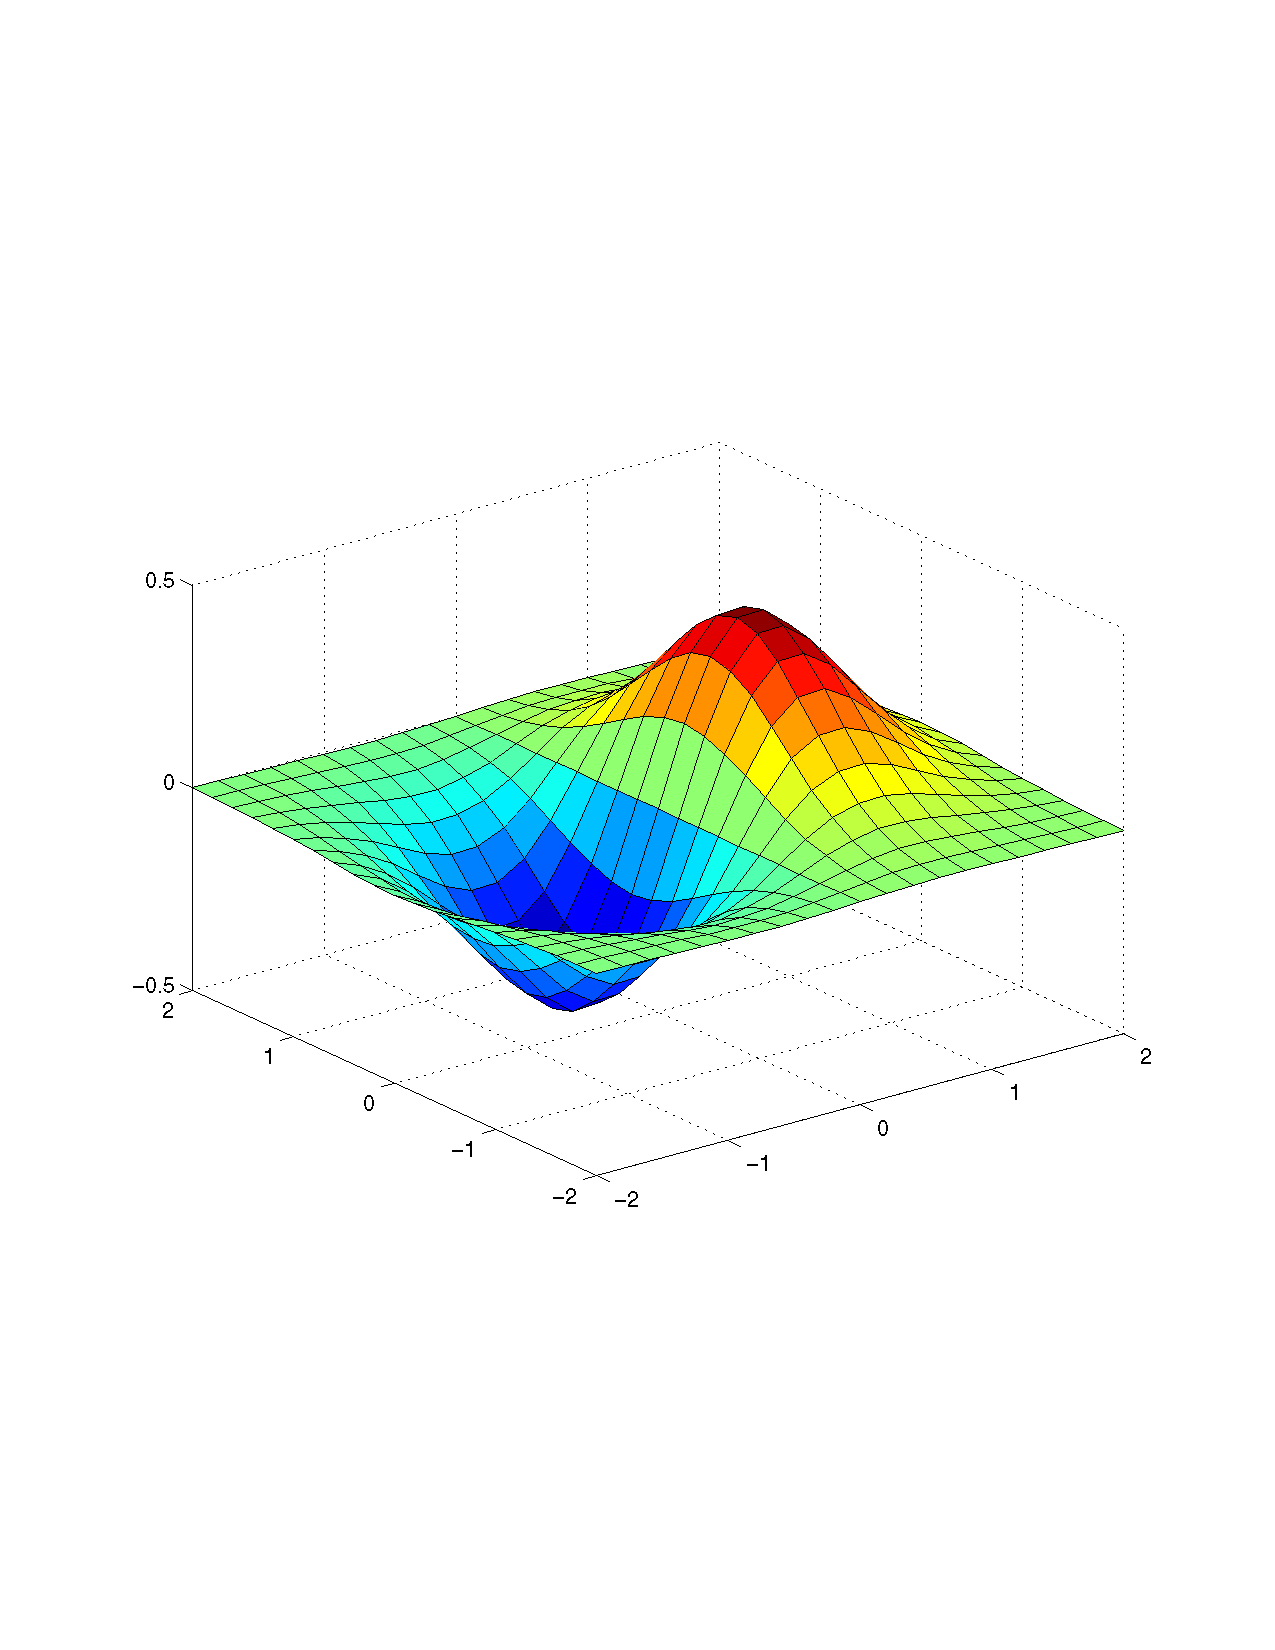
\includegraphics[width=2.5in]{./images/sample.pdf}
		\caption{My Figure 5}
		\label{fig:MyFigure5}
	\end{center}
\end{figure}

Sed adipiscing, risus vitae facilisis egestas, odio mauris sollicitudin diam, at vestibulum eros felis sed arcu. Suspendisse potenti. Sed a quam justo. Suspendisse laoreet eleifend ante, et dapibus odio bibendum nec. Aliquam viverra pellentesque est, auctor fermentum lectus tincidunt in. Praesent hendrerit purus sit amet sodales vehicula. Pellentesque vulputate fermentum justo, eget aliquam urna hendrerit ac. Ut laoreet volutpat iaculis. Duis et erat magna. Vivamus vel neque vel tortor eleifend lobortis nec sed sapien. Duis fermentum vel diam a dignissim. 

Lorem ipsum dolor sit amet, consectetur adipiscing elit. Pellentesque mattis lectus in velit facilisis lacinia. In eu bibendum lorem. Sed sollicitudin fermentum egestas. Nunc consectetur vehicula orci, eu molestie sapien sollicitudin sit amet. Phasellus sollicitudin sem quis orci aliquet, porta sagittis diam sodales. Suspendisse ullamcorper sollicitudin dictum. Donec quam sapien, molestie ut ullamcorper vitae, porttitor vitae mauris. Quisque ultrices nunc in consectetur malesuada. Pellentesque tristique purus ut felis aliquet pharetra. Mauris posuere lobortis metus id aliquam. Phasellus suscipit sapien vitae leo ultricies suscipit. Vivamus sodales egestas velit sit amet suscipit. Integer libero augue, sodales quis porta commodo, condimentum nec leo. Proin venenatis eros id venenatis facilisis.

Sed adipiscing, risus vitae facilisis egestas, odio mauris sollicitudin diam, at vestibulum eros felis sed arcu. Suspendisse potenti. Sed a quam justo. Suspendisse laoreet eleifend ante, et dapibus odio bibendum nec. Aliquam viverra pellentesque est, auctor fermentum lectus tincidunt in. Praesent hendrerit purus sit amet sodales vehicula. Pellentesque vulputate fermentum justo, eget aliquam urna hendrerit ac. Ut laoreet volutpat iaculis. Duis et erat magna. Vivamus vel neque vel tortor eleifend lobortis nec sed sapien. Duis fermentum vel diam a dignissim. 

\begin{figure}[h!]
	\begin{center}
		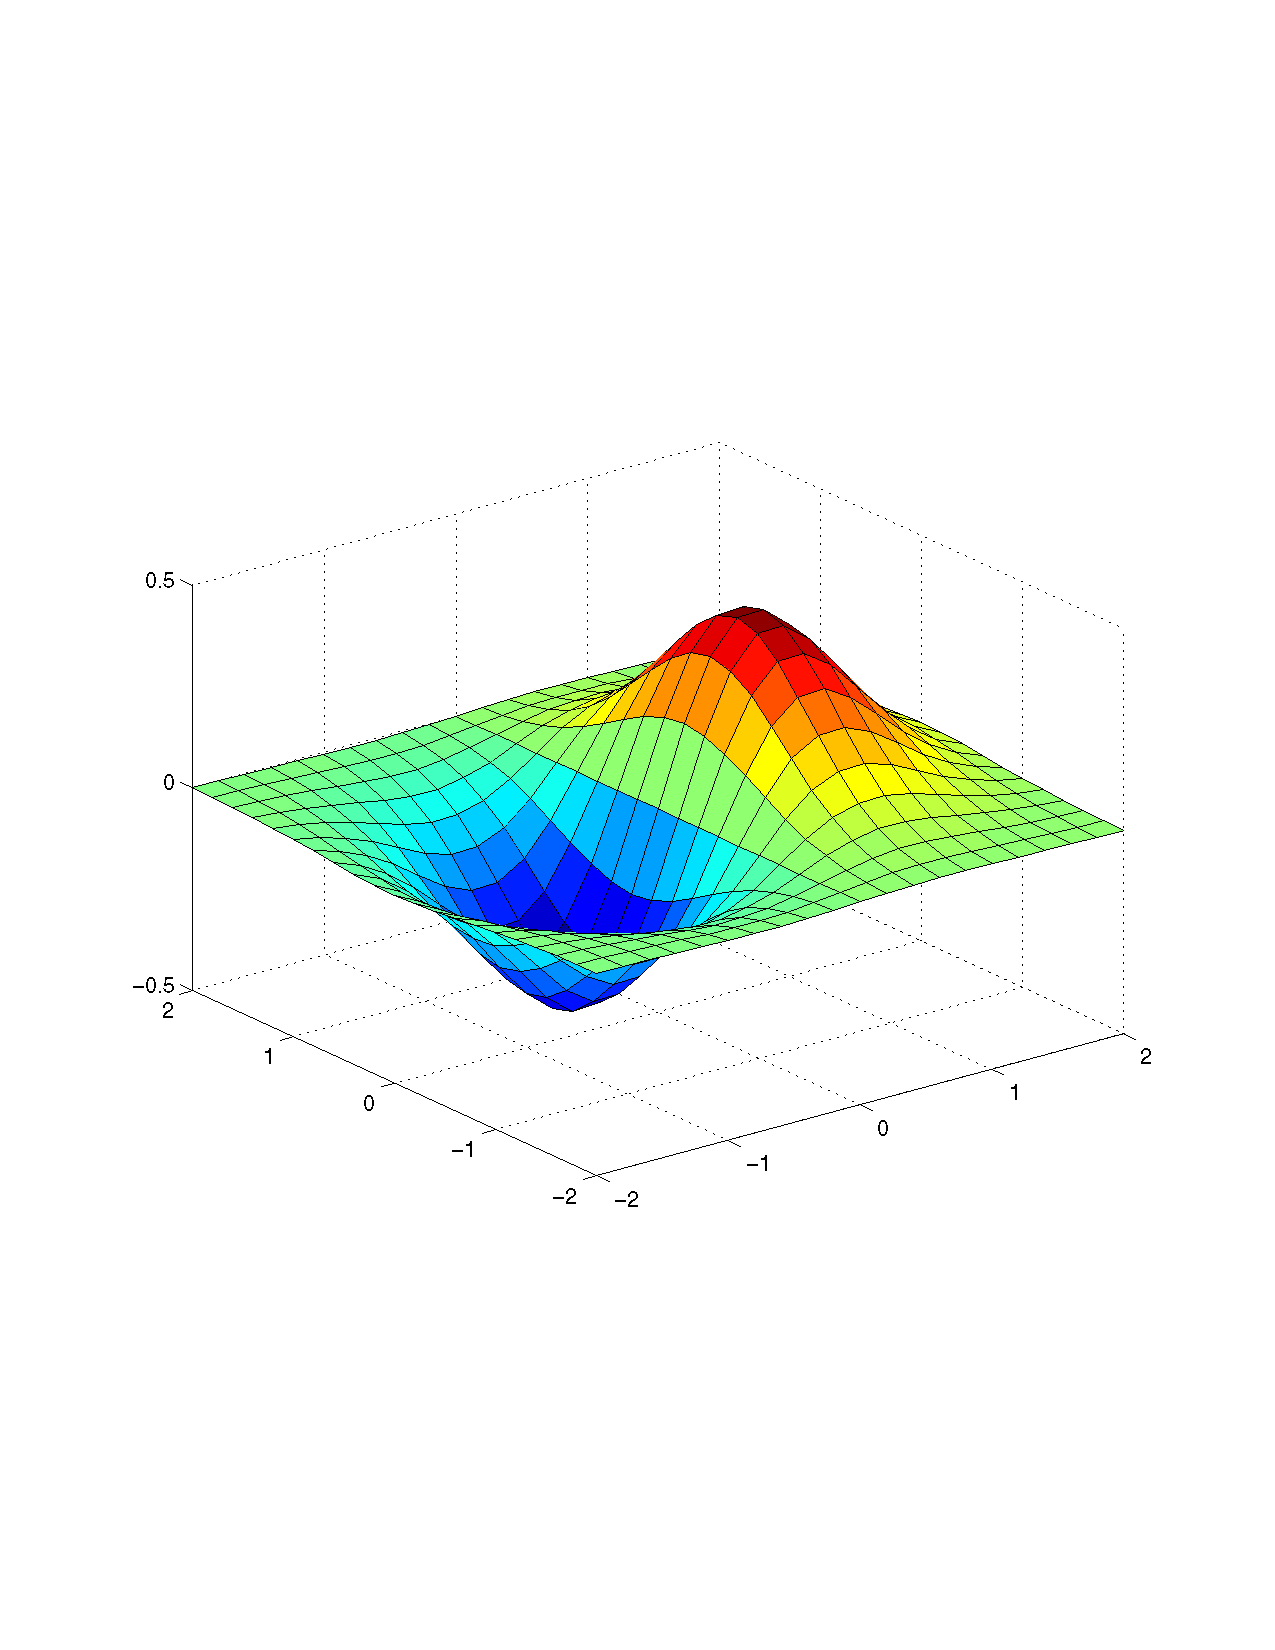
\includegraphics[width=2.5in]{./images/sample.pdf}
		\caption{My Figure 6}
		\label{fig:MyFigure6}
	\end{center}
\end{figure}

Sed adipiscing, risus vitae facilisis egestas, odio mauris sollicitudin diam, at vestibulum eros felis sed arcu. Suspendisse potenti. Sed a quam justo. Suspendisse laoreet eleifend ante, et dapibus odio bibendum nec. Aliquam viverra pellentesque est, auctor fermentum lectus tincidunt in. Praesent hendrerit purus sit amet sodales vehicula. Pellentesque vulputate fermentum justo, eget aliquam urna hendrerit ac. Ut laoreet volutpat iaculis. Duis et erat magna. Vivamus vel neque vel tortor eleifend lobortis nec sed sapien. Duis fermentum vel diam a dignissim. 

Lorem ipsum dolor sit amet, consectetur adipiscing elit. Pellentesque mattis lectus in velit facilisis lacinia. In eu bibendum lorem. Sed sollicitudin fermentum egestas. Nunc consectetur vehicula orci, eu molestie sapien sollicitudin sit amet. Phasellus sollicitudin sem quis orci aliquet, porta sagittis diam sodales. Suspendisse ullamcorper sollicitudin dictum. Donec quam sapien, molestie ut ullamcorper vitae, porttitor vitae mauris. Quisque ultrices nunc in consectetur malesuada. Pellentesque tristique purus ut felis aliquet pharetra. Mauris posuere lobortis metus id aliquam. Phasellus suscipit sapien vitae leo ultricies suscipit. Vivamus sodales egestas velit sit amet suscipit. Integer libero augue, sodales quis porta commodo, condimentum nec leo. Proin venenatis eros id venenatis facilisis.

Sed adipiscing, risus vitae facilisis egestas, odio mauris sollicitudin diam, at vestibulum eros felis sed arcu. Suspendisse potenti. Sed a quam justo. Suspendisse laoreet eleifend ante, et dapibus odio bibendum nec. Aliquam viverra pellentesque est, auctor fermentum lectus tincidunt in. Praesent hendrerit purus sit amet sodales vehicula. Pellentesque vulputate fermentum justo, eget aliquam urna hendrerit ac. Ut laoreet volutpat iaculis. Duis et erat magna. Vivamus vel neque vel tortor eleifend lobortis nec sed sapien. Duis fermentum vel diam a dignissim. 

Sed adipiscing, risus vitae facilisis egestas, odio mauris sollicitudin diam, at vestibulum eros felis sed arcu. Suspendisse potenti. Sed a quam justo. Suspendisse laoreet eleifend ante, et dapibus odio bibendum nec. Aliquam viverra pellentesque est, auctor fermentum lectus tincidunt in. Praesent hendrerit purus sit amet sodales vehicula. Pellentesque vulputate fermentum justo, eget aliquam urna hendrerit ac. Ut laoreet volutpat iaculis. Duis et erat magna. Vivamus vel neque vel tortor eleifend lobortis nec sed sapien. Duis fermentum vel diam a dignissim. 


